\documentclass[a4paper,11pt]{jsarticle}

% 数式
\usepackage{amsmath,amsfonts}
\usepackage{amsthm}
\usepackage{bm}
\usepackage{mathtools}
\usepackage{amssymb}

% 表
\usepackage[utf8]{inputenc}
\usepackage{diagbox} % 斜線付きセルを作成するために必要
\usepackage{booktabs} % 表の罫線を美しくするために必要
\usepackage{hhline} % 水平罫線を制御するために必要

% 画像
\usepackage[dvipdfmx]{graphicx}
\usepackage{ascmac}
\usepackage{physics}
\usepackage{float} % 追加

% 図
\usepackage[dvipdfmx]{graphicx}
\usepackage{tikz} %図を描く
\usetikzlibrary{positioning, intersections, calc, arrows.meta,math} %tikzのlibrary

% ハイパーリンク
\usepackage[dvipdfm,
  colorlinks=false,
  bookmarks=true,
  bookmarksnumbered=false,
  pdfborder={0 0 0},
  bookmarkstype=toc]{hyperref}

% 式番号を章ごとにリセット
\numberwithin{equation}{section}

\begin{document}

\title{情報幾何と統計力学}
\author{大上由人}
\date{\today}
\maketitle

\section{情報幾何}
\subsection{双対平坦な多様体}
狭い意味での情報幾何学として、双対アフィン接続の幾何を考える。\\

\begin{itembox}[l]{\textbf{Def:双対アフィン接続}}
    アフィン接続を持つRiemann多様体$(M,g)$に対して、双対アフィン接続$\nabla ^*$を、
    \begin{equation}
        Xg(Y,Z) = g(\nabla_X Y,Z) + g(Y,\nabla^*_X Z) \quad (X,Y,Z \in \mathfrak{X}(M))
    \end{equation}
    により定める。
\end{itembox}
例えば、Riemann接続の双対アフィン接続は、Riemann接続が計量的であることから、
\begin{equation}
    Xg(Y, Z) = g(\nabla_X Y, Z) + g(Y, \nabla_X Z) \quad (X, Y, Z \in \mathfrak{X}(M))
\end{equation}
となり、$\nabla^* = \nabla$である。(自己双対)\\
このとき、双対アフィン接続は、一意に定まることを示すことができる。また、共変微分の公理を満たすことも示される。\\

\begin{itembox}[l]{\textbf{Def:双対構造}}
    Riemann多様体$(M,g)$に対して、計量$g$に対する双対性を満たすアフィン接続のペア$(\nabla,\nabla^*)$が与えられたとき、$(g,\nabla,\nabla^*)$をMの双対構造という。
\end{itembox}

上で定義した双対接続を用いて、双対平坦な多様体の幾何を考える。特に、統計多様体においては、片方の接続が指数型分布族、もう片方の接続が混合型分布族に対応する。\\
\begin{itembox}[l]{\textbf{Def:双対平坦な多様体}}
    双対構造$(g,\nabla,\nabla^*)$を持つ多様体$(M,g)$が双対平坦であるとは、$\nabla$-曲率と$\nabla^*$-曲率がどちらも0かつ、$\nabla$-捩率と$\nabla^*$-捩率がどちらも0であることをいう。
\end{itembox}
今回は二つの接続について考えているため、それぞれの接続について局所アフィン座標系をとることができる。さらに、それぞれのアフィン座標系が、アフィン変換に対する任意性を持つことを用いると、以下の定理を示すことができる。
\begin{itembox}[l]{\textbf{Thm:局所アフィン座標系の存在}}
    双対構造$(g,\nabla,\nabla^*)$に関して平坦な多様体$M$では、各点の周りで
    \begin{equation}
        g(\partial_i,\partial_j) = \delta_{ij}
    \end{equation}
    を満たす、局所$\nabla$-アフィン座標系$(x^i)$および局所$\nabla^*$-アフィン座標系$(y^i)$の組$\{x^i,y^i\}$をとることができる。このような組$\{x^i,y^i\}$を双対アフィン座標系という。 
\end{itembox}
    
    以下では、双対 affine 座標系を用いた局所的な話に限定するため、\( U \cap V \) 自身を多様体 \( M \) とみなし、直交性をみたす大域的な \( \nabla \)-affine 座標系を \((\theta^i)\)、 \( \nabla^*\)-affine 座標系を \((\eta_j)\) で表し、それぞれ \(\theta\)-座標系、 \(\eta\)-座標系とよぶことにする。また、対応するベクトル場を
    \begin{equation}
    \partial_i := \frac{\partial}{\partial \theta^i}, \quad \partial^j := \frac{\partial}{\partial \eta_j} \tag{4.40}
    \end{equation}
    と書くことにする。また、直交性は
    \begin{equation}
    g(\partial_i, \partial^j) = \delta_i^j 
    \end{equation}
    と表すことにする。\\
    ダイバージェンスを定義する。

    \begin{itembox}[l]{\textbf{Def:ダイバージェンス}}
        $M$を、双対構造$(g,\nabla,\nabla^*)$に関する双対平坦多様体であるとする。このとき、二点$p,q \in M$に対して、定まる量
        \begin{equation}
            D(p||q) = \psi(\theta(p)) + \varphi(\eta(q)) - \theta^i(p)\eta_i(q)
        \end{equation}
        を$\nabla$-ダイバージェンスという。ただし、$\{(\theta ^i),(\eta_i)\}$は$M$の大域的な双対アフィン座標系であり、
        $\psi,\phi$は、$\eta_i = \partial_i \psi \quad \theta^i = \partial^i \varphi$を満たす。
    \end{itembox}
    定義にアフィン座標系を用いているが、結局、座標の取り方に依らないことが示される。(ここでは省略)\\
    
    $\nabla$と$\nabla^*$の役割を入れ替えると、$D(p||q)$における$\theta$と$\eta$、$\psi$と$\varphi$の役割も入れ替わる。したがって、
    \begin{equation}
        D(p||q) = D^*(q||p)
    \end{equation}
    が成り立つ。また、少し計算すると、
    \begin{align}
        D(p||q) 
        &\geq 0
    \end{align}
    かつ、
    \begin{equation}
        D(p||q) = 0 \Leftrightarrow p = q 
    \end{equation}
    が成り立つことがわかる。したがって、$D(p||q)$は、$M$上の距離のような役割を持つと考えられるが、実際には、対称性$D(p||q) = D(q||p)$は成り立たないし、三角不等式も成り立たない。したがって、$D(p||q)$は、距離の公理を満たさない。\\
    
    \textbf{ex:Euclid空間}\\
    Euclid空間においては、$\nabla = \nabla^*$である。したがって、双対平坦性はただの平坦性と帰着する。このとき、ポテンシャルは、
    \begin{align}
        \psi(z) = \varphi(z) = \frac{1}{2}\sum_{i=1}^{n} (z^i)^2
    \end{align}
    となる。したがって、ダイバージェンスは、
    \begin{align}
        D(p||q) = \frac{1}{2}\sum_{i=1}^{n} (z^i(p))^2 + \frac{1}{2}\sum_{i=1}^{n} (z^i(q))^2 - \sum_{i=1}^{n} z^i(p)z^i(q) = \frac{1}{2}\sum_{i=1}^{n} (z^i(p) - z^i(q))^2
    \end{align}
    となる。これは、Euclid空間における距離の二乗に一致する。\\
    ところで、Euclid空間において、距離の二乗と結びつく定理として、Pythagorasの定理がある。これは、双対平坦な多様体へ拡張することができる。
    
    \begin{itembox}[l]{\textbf{Thm:拡張Pythagorasの定理}}
        双対平坦多様体$(M,g,\nabla,\nabla^*)$において、点$p,q$を結ぶ$\nabla$-測地線と$q,r$を結ぶ$\nabla^*$-測地線が計量$g$に関して直交しているなら、
        \begin{equation}
            D(p||r) = D(p||q) + D(q||r)
        \end{equation}
        が成り立つ。
    \end{itembox}

\subsection{統計多様体}
情報幾何では、確率分布全体の集合を多様体として考える。
有限集合$\Omega$の要素である根元事象を自然数でラベル付けすることにして、サイズnの根元事象系を
\begin{align}
    \Omega_n = \{1,2,\cdots,n\}
\end{align}
と表すことにする。このとき、$\Omega_n$上の確率分布全体の集合を、
\begin{align}
    \mathcal{S}_n = \{p: \Omega_n \to \mathbb{R}_{++}; \sum_{\omega \in \Omega_n} p(\omega) = 1\}
\end{align}
ただし、
\begin{align}
    \mathbb{R}_{++} = \{x \in \mathbb{R}; x > 0\}
\end{align}



\begin{itembox}[l]{\textbf{Thm:Chentsovの定理}}
    Markov埋め込みの下での不変性を満たすRiemann計量は、定数倍を除いて、
    \begin{equation}
        \label{eq:Fisher1}
        g_p(X,Y) = \sum_{\omega = 1}^{n} p(\omega) (X\log p(\omega))(Y\log p(\omega))
    \end{equation}
    に限られる。一方、アフィン接続の不変性を満たすようなアフィン接続は、
    \begin{equation}    
        \label{eq:Fisher2}
        g(\nabla_X^{\alpha} Y,Z) = g(\tilde{\nabla}_X^{\alpha} Y,Z) - \frac{\alpha}{2} S_p(X,Y,Z)
    \end{equation}
    により、実数$\alpha$と一対一に対応する。ただし、
    \begin{equation}
        S_p(X,Y,Z) = \sum_{\omega = 1}^{n} p(\omega) (X\log p(\omega))(Y\log p(\omega))(Z\log p(\omega))
    \end{equation}
    である。
\end{itembox}

\begin{itembox}[l]{\textbf{Def:Fisher計量}}
    \ref{eq:Fisher1}を満たす計量$g$をFisher計量といい、\ref{eq:Fisher2}を満たすアフィン接続$\nabla^{\alpha}$を$\alpha$-接続という。

さらに、これは多様体とみなすことができ、接続および双対接続を与えることができる。この接続をそれぞれ$\nabla^{e}$、$\nabla^{m}$とする。
また、これに対応して双対アフィン座標系を導入することができる。これを$\{(\theta^i),(\eta_i)\}$とする。\\
さらに、$\nabla^*$に対応するダイバージェンスを考えることができる。

\begin{itembox}[l]{\textbf{Def.KLダイバージェンス}}
    $p,q \in \mathcal{S}_n$に対して、
    \begin{equation}
        D^m(p||q) = \sum_{\omega=1}^{n} p(\omega) \log \frac{p(\omega)}{q(\omega)}
    \end{equation}
    をKLダイバージェンスという。
\end{itembox}

また、$\mathcal{S}_n$の部分多様体として、確率関数が指数関数の形をとるものを考える。
\begin{itembox}[l]{\textbf{Def:指数型分布族}}
    $\Omega$上の関数$C(\omega),F_1(\omega),\cdots,F_k(\omega)$及び$\mathbb{R}^k$上の領域$\Theta$上を動く$k$次元パラメータ$\theta = (\theta^1,\cdots,\theta^k) \in \Theta$を用いて
    \begin{equation}
        p_{\theta}(\omega) = \exp\left[ C(\omega) + \sum_{i=1}^{k} \theta^i F_i(\omega) - \psi(\theta) \right]
    \end{equation}
    と表される確率分属族$\{p_{\theta;\theta \in \Theta}\}$を指数型分布族という。ただし、$\psi(\theta)$は、
    \begin{equation}
        \psi(\theta) = \log \left[ \sum_{\omega \in \Omega} \exp\left[ C(\omega) + \sum_{i=1}^{k} \theta^i F_i(\omega) \right] \right]
    \end{equation}
    で定義される。  
\end{itembox}
この量が、確率分布間の距離(のようなもの)として、対応してくれる。\\

上の定義で与えた指数型分布族を$M$とする。また、指数型分布族から一旦視点を$\mathcal{S}$に戻してあげて、

統計多様体$(\mathcal{S},g,\nabla^{e},\nabla^{m})$の$\nabla^{e}$-自己平行部分多様体である指数型分布族
\begin{equation}
    M = \{p_{\theta}(\omega) \in \mathcal{S}; \log p_{\theta}(\omega) = C(\omega) + \sum_{i=1}^{k} \theta^i F_i(\omega) - \psi(\theta) \}
\end{equation}
が与えられたとする。$M$の期待値座標系を固定したときに定まる$\mathcal{S}$確率分布族
\begin{equation}
    \Gamma_{\eta} = \{q(\omega) \in \mathcal{S}; E_q [F_i] = \eta_i \}
\end{equation}
を考える。

\begin{itembox}[l]{\textbf{Thm:}}
    $M$と$\Gamma_{\eta}$が共有点を持つならば、その点において、$M$と$\Gamma_{\eta}$は直交する。
\end{itembox}


\section{統計力学}
\subsection{エントロピー最大原理}
統計力学における各分布の構成方法として、シャノンエントロピーを適当な拘束条件の元で最大化する方法がある。

エネルギー期待値を一定に保った時の、シャノンエントロピー最大化問題を考える。シャノンエントロピーは確率分布関数の汎関数であるから、変分によって停留点を探す。
\begin{align}
  \tilde{S}= -k_B\sum_{i}p_i\log p_i -\lambda\left(\sum_{i}p_i - 1\right)-\rho\left(\sum_{i}p_iE_i - U\right)  
\end{align}
である。ここで、$\lambda$と$\rho$は未定乗数である。微小な確率変分を考えると、
\begin{align}
  \delta \tilde{S} &= -k_B\sum_{i}(p_i + \delta p_i)\log (p_i + \delta p_i) -\lambda\left(\sum_{i}(p_i + \delta p_i)- 1\right) -\rho\left(\sum_{i}(p_i + \delta p_i)E_i - U\right)-\tilde{S}\\
  &= -k_B\sum_{i}\left(\delta p_i\log p_i + (p_i + \delta p_i)\log \left(1 + \frac{\delta p_i}{p_i}\right)\right)  -\lambda\left(\sum_{i}\delta p_i\right)-\rho\left(\sum_{i}\delta p_iE_i\right)
\end{align}
となる。ここで、$\log(1+x) = x + O(x^2)$であることを用いて、
\begin{align}
  \delta \tilde{S} &= -k_B\sum_{i}\left(\delta p_i\log p_i + \delta p_i\right)  -\lambda\left(\sum_{i}\delta p_i\right)-\rho\left(\sum_{i}\delta p_iE_i\right)\\
  &= \sum_{i}\delta p_i\left(-k_B\log p_i - k_B - \lambda - \rho E_i\right) + O(\delta p_i^2)
\end{align}
となる。したがって、
\begin{align}
  -k_B\log p_i - k_B - \lambda - \rho E_i = 0
\end{align}
である。これを変形して、
\begin{align}
  p_i = \exp(-1-\frac{\lambda}{k_B}-\frac{\rho E_i}{k_B})
\end{align}
したがって、
\begin{align}
  p_i \propto \exp(-\beta E_i)
\end{align}
となる。ここで、$\beta = \frac{1}{k_B T}$である。($\rho = \frac{1}{T}$)\\
あとは、規格化条件から、
\begin{align}
    p_i &= \frac{1}{Z} \exp(-\beta E_i)\\
    Z &= \sum_{i} \exp(-\beta E_i)
\end{align}
であることがわかる。これがカノニカル分布である。\\

\subsection{KLダイバージェンス最小化}
統計力学における最大エントロピー原理は、情報幾何の立場では、一様分布とのKLダイバージェンスを最小化することに対応する。\\

カノニカル分布の形を思い出しつつ、指数型分布族において、$k=1$とし、$F_1(\omega) = -H(\omega)$とする。そして、$\theta = 0$で一様分布
\begin{equation}
    u = \qty(\frac{1}{n},\cdots,\frac{1}{n})
\end{equation}
を通る1次元指数型分布族($\nabla^{e}$-測地線)を考える。このとき、この測地線は、
\begin{align}
    p_{\theta}(\omega) &= \exp\left[ -\theta H(\omega) - \psi(\theta) \right]
\end{align}
となる。\footnote{$\theta = 0$で一様分布になってほしいので、$C(\omega)=0$とする。}このとき、この測地線と、
\begin{equation}
    \Gamma_{\eta} = \{q \in \mathcal{S}; E_q[-H] = \eta \}
\end{equation}
は直交する。

一般化Pythagorasの定理より、
\begin{align}
    p_{\theta_*} &= \underset{q \in \Gamma_\eta}{\text{argmin}} \qty{D^e(u||q)} \\
    &= \underset{q \in \Gamma_\eta}{\text{argmin}} \qty{D^m(q||u)}\\
    &= \underset{q \in \Gamma_\eta}{\text{argmin}} \sum_{\omega \in \Omega} q(\omega) \log \frac{q(\omega)}{u(\omega)}\\
    &= \underset{q \in \Gamma_\eta}{\text{argmin}} \{\log n -S(q)\}\\
    &= \underset{q \in \Gamma_\eta}{\text{argmax}} \{S(q)\}
\end{align}
となる。これは、確率変数$F_1(\omega) = -H$の期待値が一定であるもとで、Shanonエントロピー$S(q)$を最大にする確率分布は、
$\Gamma_{\eta}$から測地線に下した垂線の足$P_{\theta_*}$に一致することを示している。

\begin{figure}[H]
    \begin{center}
    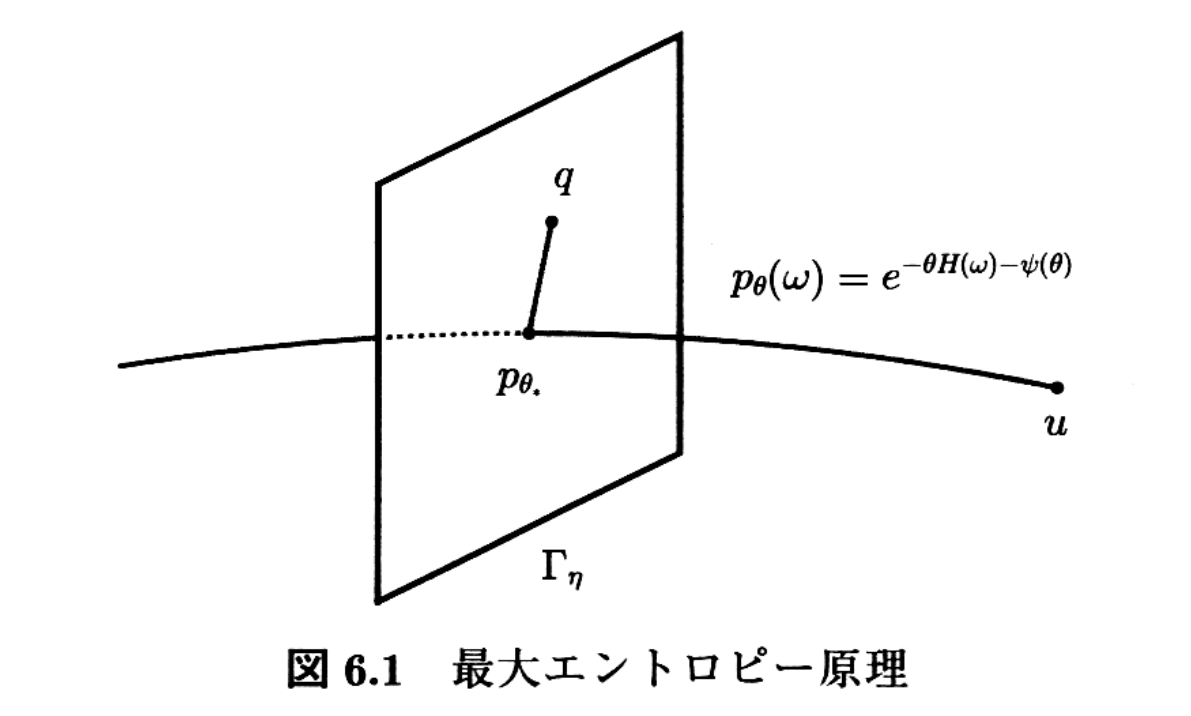
\includegraphics[width=100mm]{entropy.png}
    \end{center}
    \caption{エネルギー期待値が一定の面の中で一様分布に最も近い分布が$p_{\theta_*}$である。}
    \label{fig:one}
\end{figure}


\end{document}